\documentclass{article}
\usepackage[utf8]{inputenc}
\usepackage[T5]{fontenc}
\usepackage{graphicx}
\usepackage[margin=2cm]{geometry}
\title{Report 4: Threads}
\author{Nguyễn Thanh Hùng -- 2540056}
\date{October 8, 2026}

\begin{document}
\maketitle

\section{Implementation}
I changed the grayscale kernel to use 2D blocks. Thread $(x,y)$ processes pixel $(y,x)$. I compared 1D and 2D kernels with the same number of threads per block.

I ran the notebook on Google Colab with a Tesla T4 and a $256\times256$ sample image.
GPU timings use \texttt{time.time()} after warm-up and synchronization, averaged over three runs; allocation and image transfers are excluded. Where measured, CPU time is one run; speedup is relative to that Python CPU implementation.

\section{Results}
CPU time: 463.1267 ms. Maximum pixel error: 1.
\begin{center}
\begin{tabular}{lrr}
\hline
2D block & 1D GPU (ms) & 2D GPU (ms) \\
\hline
(8, 8) & 0.0769 & 0.0572 \\
(16, 16) & 0.0405 & 0.0561 \\
(32, 16) & 0.0501 & 0.0513 \\
(32, 32) & 0.0550 & 0.0743 \\
\hline
\end{tabular}
\end{center}\begin{center}
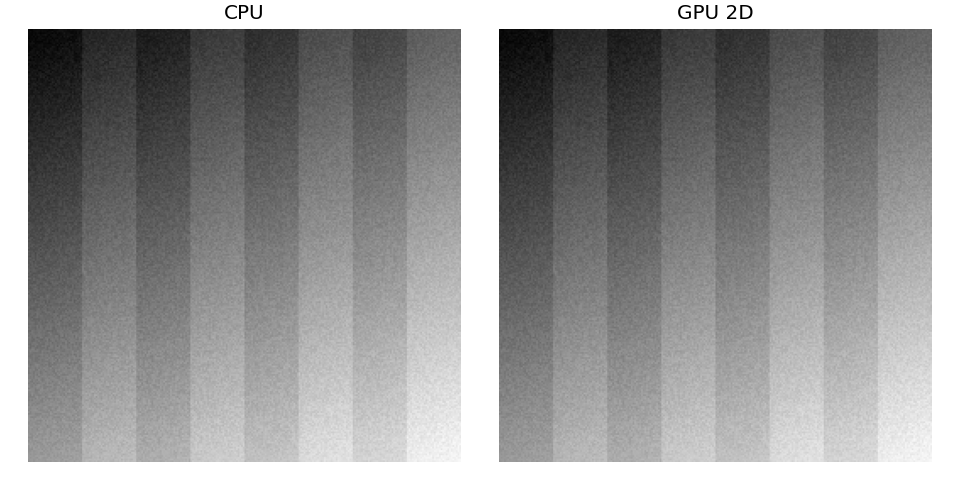
\includegraphics[width=.48\linewidth,height=.15\textheight,keepaspectratio]{figures/images.png}
\hfill
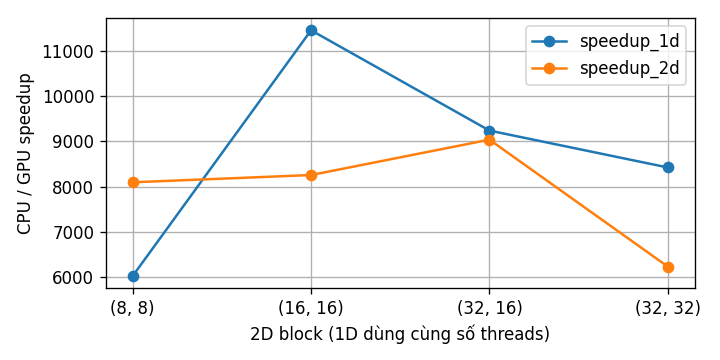
\includegraphics[width=.48\linewidth,height=.15\textheight,keepaspectratio]{figures/performance.png}
\end{center}

\section{Discussion}
The best 1D time was 0.0405 ms with 256 threads; the best 2D time was 0.0513 ms with a $32\times16$ block. Their CPU/GPU speedups were 11449 and 9035. The 2D kernel is not always faster.

\section{Exercises}
\begin{itemize}\setlength{\itemsep}{0pt}
\item Exercise 1: choose $16\times16$. Four blocks give 1024 threads/SM. An $8\times8$ block gives only 512 threads with eight blocks; $32\times32$ exceeds the stated 512-thread block limit.
\item Exercise 2: 128, 256, 512 and 1024 threads/block give 512, 1024, 1536 and 1024 resident threads. Choose 512 threads/block.
\item Exercise 3: $\lceil2000/512\rceil=4$ blocks launch 2048 threads; 48 threads have no element to process.
\end{itemize}
These are the hypothetical exercise limits, not the Tesla T4 limits.

\end{document}
